\section{Design}\label{sec: Design}
In this section the design and decisions that where made to achieve the laboratory are discussed.

\subsection{SDK}\label{subsec: SDK}
As software development kit (SDK) the Spyder IDE is used that is part of the anaconda navigator which provides the Python 3.7 interpreter and default packages. This installation makes it very easy for a beginner to start with python programming. The Spyder IDE is shown in Figure \ref{fig: SpyderIDE}. Highlighted are the python version on top, the debug run button to execute a script in console, and the console to make input and outputs to the script. Notice tis is not a program it is a script.
\begin{figure}[H]
	\centering
	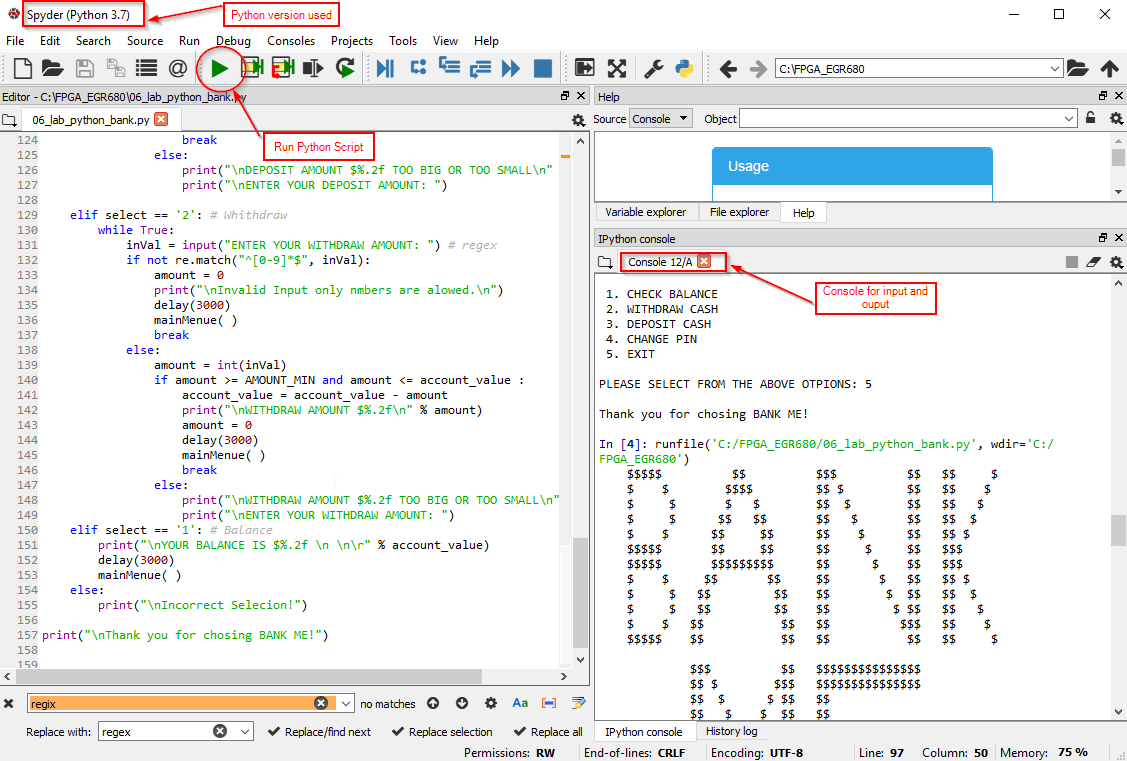
\includegraphics[width=1.0\textwidth]{01_images/SpyderIDE.PNG}
	\caption{Shows the Spyder IDE with the most important information highlighted.}
	\label{fig: SpyderIDE}
\end{figure}



\subsection{ATM machine}\label{subsec: Lab specification}
Part III states to program an ATM machine with input and output in the command line or python IDLE environment. The user input validation is done with with regex so that each input is restricted to a specific set of characters in combination with a while loop, as shown in Listing \ref{lst: Python code for input validation}. The function used for regex is re.match() and is imported with the package re. To build and test a regex a vast amount of on-line tools are available as the one the author used was \href{http://regex101.com/}{regex101.com}.

\begin{lstlisting}[style=PythonStyle, language=Python, caption={Python code for input validation.},label=lst: Python code for input validation]
# PIN validation
while True:
	inVal = input("Please enter your PIN: ") # regex
	if not re.match("^[0-9]{4}$", inVal):
		print ("Error! Make sure you only use numbers from 0-9 in PIN")
		inVal = 'Z'             
	else:
		if inVal == PIN :    
			#print("\nCorect PIN") # debug only
			inVal = 'Z'  
			break             
		else:        
			print("\nInvalid PIN!")
			inVal = 'Z'  
\end{lstlisting}

Python allows to make functions as in C, a function definition is shown in Listing \ref{lst: Python code for delay}. First the time package was imported but with the function sleep the problem is it stop's the thread before the print output to the console was made. therefore a simple for loop was used and approximated to one second which is not precious but does the job. Furthermore a variable in python can be referenced to any data type.
\begin{lstlisting}[style=PythonStyle, language=Python, caption={Python code for delay.},label=lst: Python code for delay]
def delay( msec ):
	cnt = 0
	while cnt < msec:
		cnt += 0.0001
		return
\end{lstlisting}

The ATM machine is first welcoming the user with the name of the Bank and a Welcome message. Below the user is ask to identify himself with his personal identification number (PIN) which will allow the user access to his account if entered correctly. Followed by prompt of the Main Menu as shown in Figure \ref{fig: MainMenu}. The user can use the keyboard to make a selection of the task he wants do to. The figure shows highlighted where the user made an input selection of no. five and the output generated by the script exiting the users individual secure area. As long as the user does not exit he can proceed with all actions presented in the main menu. A demonstration of the functionality will be given to the instructor in class.
\begin{figure}[H]
	\centering
	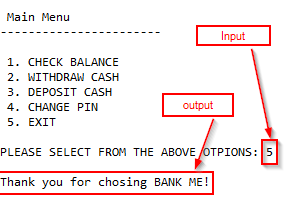
\includegraphics[width=0.5\textwidth]{01_images/MainMenu.PNG}
	\caption{Main menu with highlighted user input and program output.}
	\label{fig: MainMenu}
\end{figure}


